\documentclass[12pt, twoside, openright]{book}
\usepackage{graphicx} % Required for inserting images
\usepackage[letterpaper,width=150mm,top=25mm,bottom=25mm]{geometry}
\usepackage{setspace}\onehalfspace
%\setstretch{1.5}
\usepackage[utf8]{inputenc}
\usepackage[T1]{fontenc}
\usepackage{url}
\usepackage[spanish]{babel}
\usepackage[textsize=tiny, colorinlistoftodos]{todonotes}
\usepackage[%
backend=biber,
natbib=true,
style=apa,
]{biblatex}
%\usepackage{apacite}
%\usepackage{fullpage}
\usepackage[Sonny]{fncychap}

%\newcommand{\quentin}[2][]
%{\todo[author=Quentin, color=green!40, #1]{#2}}

\title{Templete seminario de tesis}
\author{Abraham Olivetti}
\date{Octubre 2023}


\addbibresource{biblio.bib}

\begin{document}

\clearpage{\pagestyle{empty}\cleardoublepage} %Para agregar una página en blanco después de las secciones.
\maketitle
\clearpage{\pagestyle{empty}\cleardoublepage}
\tableofcontents
\clearpage{\pagestyle{empty}\cleardoublepage}


%Aquí los capítulos%
\chapter*{Introducción}

\noindent The importance of the role that conditionals play in both everyday and scientific discourse and reasoning is hard to overestimate.
Perhaps it is no surprise then that for quite some time, conditionals have been a central area of investigation not only in philosophy, but also in linguistics and psychology, and to some extent in computer science.
What is surprising, however, is that despite the considerable expenditure of time and effort of many researchers from those fields, there is still little that one can say about conditionals that is not highly controversial. 
Even with regard to the most fundamental questions concerning conditionals, there is very little unanimity to be found. 
Those who have ever proposed a semantics of conditionals can consider themselves fortunate if the proposal won the approval of at least one colleague. %Esto es un comentario, no va a aparecer en el pdf compilado


Ejemplo para ver si funciona git push

\clearpage{\pagestyle{empty}\cleardoublepage} %Esto elimina los números de las páginas en blanco
\pagestyle{headings}%esto reinserta los números de las páginas y los encabezados

\chapter{Introducción}
\noindent Aquí un breve resumen de lo que va a tratar el capítulo

\section{Condicionales}

\noindent The importance of the role that conditionals play in both everyday and scientific discourse and reasoning is hard to overestimate. \citep{Ariotti1968} %Esto es una cita
Perhaps it is no surprise then that for quite some time, conditionals have been a central area of investigation not only in philosophy, but also in linguistics and psychology, and to some extent in computer science.
What is surprising, however, is that despite the considerable expenditure of time and effort of many researchers from those fields, there is still little that one can say about conditionals that is not highly controversial. 
Even with regard to the most fundamental questions concerning conditionals, there is very little unanimity to be found. 
Those who have ever proposed a semantics of conditionals can consider themselves fortunate if the proposal won the approval of at least one colleague. %Esto es un comentario, no va a aparecer en el pdf compilado

\subsection{Más sobre condicionales}

\noindent This book focusses on the distinctively epistemological questions that conditionals raise, such as questions concerning their acceptability conditions and probabilities.
There is hardly more consensus on these epistemological questions than there is on the semantics of conditionals.
And insofar as there is consensus, it is based on questionable assumptions.
In this book, I aim to develop at least an outline of the epistemology of conditionals. 
I do so by relying on the combined use of formal and empirical methods.

%esto es una cita en bloque
\begin{quote}
    This book focusses on the distinctively epistemological questions that conditionals raise, such as questions concerning their acceptability conditions and probabilities.
    There is hardly more consensus on these epistemological questions than there is on the semantics of conditionals.
    And insofar as there is consensus, it is based on questionable assumptions.
    In this book, I aim to develop at least an outline of the epistemology of conditionals. 
    I do so by relying on the combined use of formal and empirical methods. \citep{Blaasjoe2022}
\end{quote}

\subsection{Repetido lo anterior, sólo para ver los encabezados}

\noindent The importance of the role that conditionals play in both everyday and scientific discourse and reasoning is hard to overestimate. \citep{Ariotti1968} %Esto es una cita
Perhaps it is no surprise then that for quite some time, conditionals have been a central area of investigation not only in philosophy, but also in linguistics and psychology, and to some extent in computer science.
What is surprising, however, is that despite the considerable expenditure of time and effort of many researchers from those fields, there is still little that one can say about conditionals that is not highly controversial. 
Even with regard to the most fundamental questions concerning conditionals, there is very little unanimity to be found. 
Those who have ever proposed a semantics of conditionals can consider themselves fortunate if the proposal won the approval of at least one colleague. %Esto es un comentario, no va a aparecer en el pdf compilado
The importance of the role that conditionals play in both everyday and scientific discourse and reasoning is hard to overestimate. \citep{Ariotti1968} %Esto es una cita
Perhaps it is no surprise then that for quite some time, conditionals have been a central area of investigation not only in philosophy, but also in linguistics and psychology, and to some extent in computer science.
What is surprising, however, is that despite the considerable expenditure of time and effort of many researchers from those fields, there is still little that one can say about conditionals that is not highly controversial. 
Even with regard to the most fundamental questions concerning conditionals, there is very little unanimity to be found. 
Those who have ever proposed a semantics of conditionals can consider themselves fortunate if the proposal won the approval of at least one colleague. %Esto es un comentario, no va a aparecer en el pdf compilado


\section*{Conclusiones} %el asterisco es para que no numere la sección

\noindent Aquí un breve repaso de lo que hicieron en este capítulo y cuál fue la premisa defendida.
\clearpage{\pagestyle{empty}\cleardoublepage}
\pagestyle{headings}
\chapter{Introducción}
\noindent Aquí un breve resumen de lo que va a tratar el capítulo

\section{Condicionales}

\noindent The importance of the role that conditionals play in both everyday and scientific discourse and reasoning is hard to overestimate.\footnote{Esto es una nota al pie}
Perhaps it is no surprise then that for quite some time, conditionals have been a central area of investigation not only in philosophy, but also in linguistics and psychology, and to some extent in computer science.
What is surprising, however, is that despite the considerable expenditure of time and effort of many researchers from those fields, there is still little that one can say about conditionals that is not highly controversial. 
Even with regard to the most fundamental questions concerning conditionals, there is very little unanimity to be found. \citep{aristotelesnico}
Those who have ever proposed a semantics of conditionals can consider themselves fortunate if the proposal won the approval of at least one colleague. %Esto es un comentario, no va a aparecer en el pdf compilado

\subsection{Más sobre condicionales}

\noindent This book focusses on the distinctively epistemological questions that conditionals raise, such as questions concerning their acceptability conditions and probabilities.
There is hardly more consensus on these epistemological questions than there is on the semantics of conditionals.
And insofar as there is consensus, it is based on questionable assumptions.
In this book, I aim to develop at least an outline of the epistemology of conditionals. 
I do so by relying on the combined use of formal and empirical methods. 


%La h es para poner la imagen 'aquí' mliteralmente 'here'. 'width' y 'height' son valores para el tamaño de la imagen. \caption{*} es para poner pie uy número a la imagen 
\begin{figure}[h]
    \centering
    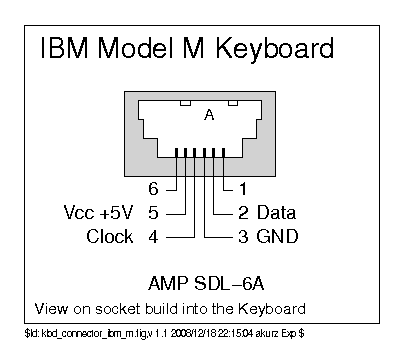
\includegraphics[width=5cm, height=5cm]{./Imágenes/kbd_connector_ibm_m.png}
    \caption{La condenada entrada SDL}
    \label{fig:sdl1}
\end{figure}

\section*{Conclusiones} %el asterisco es para que no numere la sección

\noindent Aquí un breve repaso de lo que hicieron en este capítulo y cuál fue la premisa defendida. una referencia a la imagen \ref{fig:sdl1}
\clearpage{\pagestyle{empty}\cleardoublepage}

%bibliografía
\printbibliography

\end{document}
